\chapter{Related Work} \label{related_work}
 

In this chapter we briefly discuss two similar bubble measurement techniques that aim to estimate bubble concentrations in water. The first is a master's thesis by \citep{Leonie}, where a bright field method was used in a wind wave facility, so that bubbles appeared as dark circles on camera, and the second is a field measurement technique \citep{Al-Lashi2016}, where bubbles were artificially lit from below, yielding similar images to our own. 

\section{Bright field method}
	As an improved method from \citet{MischlerDiss}, this technique uses a bright field method as shown in figure \ref{fig:bright_field}. Bubbles in this experimental setup are backlit, so that they appear completely dark except for one spot in the center (see section  \ref{bubble_physics}). Note the need to use a lens shift adapter because the incoming rays are not parallel. 
	
		\begin{figure}
			\centering
			\begin{subfigure}[t]{0.55\textwidth}
				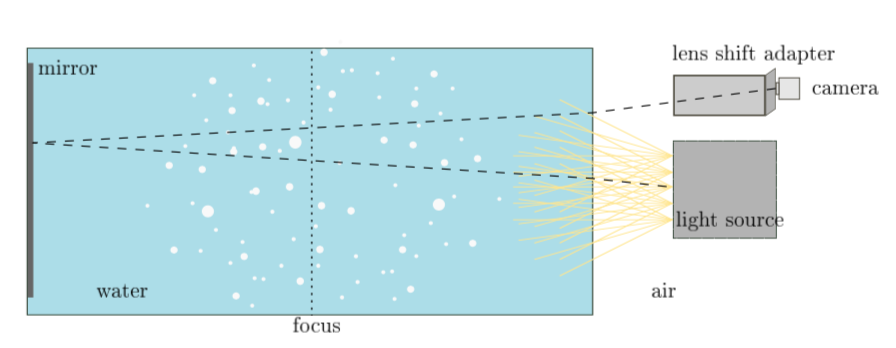
\includegraphics[scale=.4]{images/bright_field_method.png}
				\caption{Experimental setup of a light field method at Aeolotron facility}
			\end{subfigure}
			
			\begin{subfigure}[t]{0.3\textwidth}
				\centering
				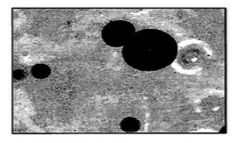
\includegraphics[scale=0.5]{images/bright_field_result.png}
				\caption{Sample result image}
			\end{subfigure}%
			\begin{subfigure}[t]{0.3\textwidth}
				\centering
				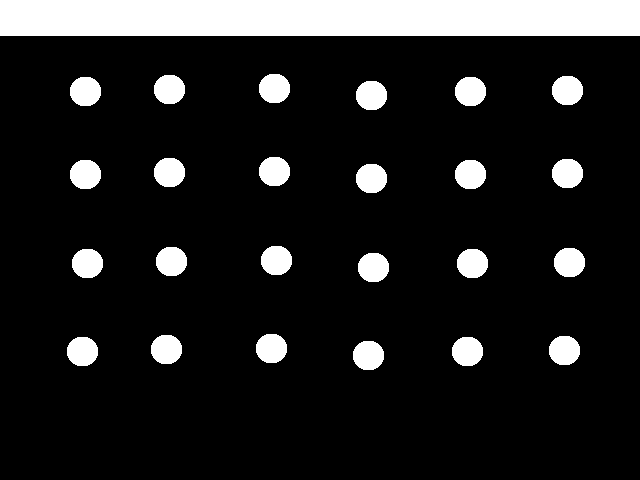
\includegraphics[scale=0.15]{images/bright_field_calibration_target.png}
				\caption{calibration target}
				\label{subfig:calib_target}
			\end{subfigure}
			
			\caption{Bright field method}
			\label{fig:bright_field}
		\end{figure}		
	
	Depth of field calibration was based on the edges between bubbles and background. The higher the edge's magnitude, the closer the bubble is to the focus plane. A calibration target made of hollow circles was used to calibrate the depth of field (figure \ref{subfig:calib_target}). 
	
	The images obtained by this method are arguably the most important advantage of this technique, since it reduces bubbles to simple circles, making them relatively easy to detect, whereas our algorithms need to recognize significantly more complex patterns than mere circles.
	 In contrast to our method however, the bright field technique constrains how close the camera can get to the water surface. Also, \citet{Leonie} does not define a criteria that measures how well the circle detection algorithm performs, so the assumption is that precision is close to perfect, which introduces an error to bubble concentration measurement that was essentially neglected. 
	 Nevertheless, this work was very important for our newly developed method because it offered an estimation of boundary conditions, such as the largest possible bubble radius and the largest possible bubble concentration, that were important to determine the different hyperparameters of our algorithm and therefore contributing to the accuracy of our algorithms. 
	
	
\section{Bubble optical imaging instrument}
	This technique submerges an optical imaging instrument (figure \ref{subfig:optical_imaging}) underwater and illuminates a thin slice	of water of volume 4cm $\times$ 4cm $\times$ 5mm. This method is particularly interesting because it produces images similar to our own. However, applying the algorithm from this paper did not yield good results. This is most likely due to the fact that our method does not illuminate the bubbles from above, making the bubble's circular shape not easily detectable with a Hough transform \citep{Hough1972} \citep{Al-Lashi2016}.
	
		\begin{figure}[h]
			\centering
			\begin{subfigure}[t]{0.4\textwidth}
				\centering
				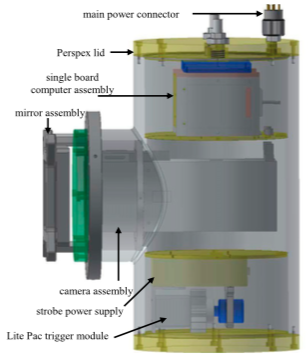
\includegraphics[scale=.3]{images/bubble_optical_imaging_instrument.png}
				\caption{Bubble optical imaging instrument. The submerged device }
				\label{subfig:optical_imaging}
			\end{subfigure}\hfill
			\begin{subfigure}[t]{0.4\textwidth}
				\centering
				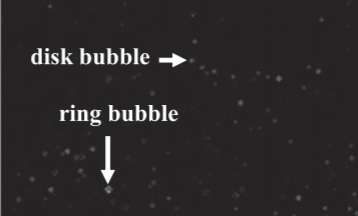
\includegraphics[scale=.5]{images/sample_result_optical_imaging_instrument.png}
				\caption{Sample result image containing two types of bubbles: filled circles (disks) and rings. }
				\label{subfig:result_optical_imaging}
			\end{subfigure}
			\label{fig:optical_imaging}
			\caption{Bubble detection with the bubble optical imaging instrument}
		\end{figure}		























